%%% -*-LaTeX-*-

\chapter{Methods}\label{methods}

The purpose of this study is to develop an interpretable machine learning (ML)
model to efficiently compute stress intensity factors (SIFs) from stresses in
1D line weld elements given user-defined initial crack sizes.  The SR model acts
as a low-fidelity surrogate model, mapping line-weld element stresses within a
structural-element model to the SIFs computed from a crack inserted into a
matching solid-element model. This process ensures that engineering
frameworks can utilize highly efficient line weld elements but
still model higher-fidelity 3D crack growth estimates.  A high-level workflow of
the process is shown in Figure \ref{fig:workflow} to illustrate the overall
dataflow. A brief overview of the process is given next, followed by a detailed
discussion of each box in Figure \ref{fig:workflow} in the following
subsections.

As discussed in Section \ref{introduction}, line-weld elements are used in
engineering applications because of their computational efficiency.  However,
because they are 1D, cracks cannot be modeled geometrically, and corresponding
SIFs cannot be computed. For this reason, two models are developed for the same
structural joint. In the first, solid finite elements are used wherein
arbitrary 3D crack surfaces can be geometrically represented and SIFs computed.
In the second, the more efficient structural finite elements, shells and line
welds are used. In this manner, SIFs from the first model (solid elements)
are provided for the second model (structural elements) with matching boundary
conditions and stress states.  

To ensure an adequate match between the solid- and structural-element models,
limits on the applied BCs are determined (box 1), discussed in Section
\ref{fem}.  Next, a sensitivity analysis is performed to provide an initial
guideline for the variation of BCs that must be applied to generate adequate
training data for the ML model (box 2).  At this point, crack growth is
simulated in the solid-element model using Abaqus and FRANC3D to generate the training
data for the applied BCs, crack size, and resulting SIFs (box 3).  Concurrently,
the shell models with line weld elements are simulated with the same BCs to
generate training data for the line weld element stresses (box 4).  At this
stage, the training features are the line weld stresses and crack sizes, while
the training label is the computed SIFs.  These training data are then provided
to the Bingo software for interpretable ML model generation (box 5).  The output
of this process is a ML model, which takes as inputs the crack size and line weld
stresses and returns a SIF estimate, as would be computed by a 3D solid element
model (box 6).  

There are assumptions we are making to map SIFs from stresses in the line-weld element. We know that as a crack grows, the stresses around the crack redistribute. However, in our model, the local stresses in the line-weld are constant for each combination of BCs. Therefore our model assumes negligible stress redistribution as the crack evolves.

\section{Finite Element Models} \label{fem}

The geometry shown in Figure \ref{fig:abaqus_model} represents a C-channel
welded to a plate. The weld is 3 mm thick and creates a gap of 0.05 mm between
the web of the C-channel and the plate. The C-channel is idealized as a constant
thickness. The channel, plate, and weld are treated as one material, and the weld
is idealized as having no heat-affected zone. As discussed above, a
solid-element model of this geometry was generated to compute SIFs for arbitrary
3D cracks initiating at the weld, while the engineering analyses are expected to
utilize a shell-element model of this geometry.  Consequently, to acquire
representative SIFs for the shell-element model, a mapping between the shell and
solid models based on a stress resultant is required.  This ensures that
the SIFs acquired from the solid model match the stress state of the shell model
being analyzed.  Therefore, to enable this mapping, the first task was to develop
matching shell- and solid-element models. 

FRANC3D uses quarter-point wedge elements along the crack front, and the
remaining elements throughout the volume are quadratic tetrahedral elements. For
this reason, quadratic tetrahedral elements were used in the solid-element
model, which is remeshed during crack growth using FRANC3D. The solid-element
model contains approximately 1e6 quadratic tetrahedral elements.  This number of
elements was found to be more than sufficient after a convergence study on
maximum principal stresses on the weld surface. The higher number of elements
was used because smaller elements were needed to facilitate crack insertion on
the weld surface.  

To be more computationally efficient, Franc3D allows one to subdivide a model to
operate more efficiently on a smaller region. This allows for the remeshing to
happen faster and results in fewer elements in the global model. A cube of
side length 12.7 mm from the weld region is extracted with a finer mesh to be
subject to crack insertion and growth. Moreover, this cube is focused at
mid-span of the weld and aligned with the line-weld element in the shell element
model that will provide local stress-resultants. Within this partition is a
smaller partition with an even finer mesh to allow for a 0.05 mm crack to be
inserted into the mesh by FRANC3D.

The shell-element model contains shell elements and line-weld elements. The
length and width of the plate and C-channel are the same as in the 3D model.
The C-channel connects to the plate with a set of 1D line-weld elements to
manage a contact relationship between edges of the C-channel shell mesh and
surfaces of an adjacent plate shell mesh. Line-weld elements consist of a block
of truss elements, and a side set made up of shell elements. Line welds have 4
degrees of freedom: r, s, t, and moment-about r denoted l. r represents shear on
the surface, in the direction of the weld, s represents shear on the surface,
normal to the weld, and t represents tearing away from the surface. These local
coordinates are illustrated in Figure \ref{fig:local_coords}. The shell elements
model is simulated using Sandia’s SIERRA Mechanics software \cite{osti_1433781}
because of its ability to model line-weld elements.

Displacement BCs were applied to the shell and solid FE models.  The BCs
exercise each of the r, s, t, and l deformation modes.  An initial study was
completed to adjust the maximum value of each applied BC such that there was not
one mode that dominated the response of the model.  The numbering of the
surfaces is illustrated in Figure \ref{fig:surface_nums}. For r-loading,
surfaces 6 and 60 are displaced in the positive z-direction. For s-loading,
surface three is displaced in the positive x-direction. For t-loading, surfaces
4 and 40 and displaced in the positive y-direction. Finally, for l-loading, surface
four is displaced in both the positive and negative x-direction. 

The shell-element model utilized here inherently uses nonlinear geometry. However, the solid model did not include nonlinear geometry to save a substantial amount of computing time. Consequently, with increased applied BC values, the
results of the shell and solid models were observed to diverge.  It was decided
that, to limit this discrepancy, the applied BC values would be limited, such
that a difference of less than 1\% in resultant displacement between the shell
and solid model was observed, see Figure \ref{fig:workflow}.  In some cases, the
applied BC limits were further reduced to ensure that a single applied BC would
not dominate the maximum principal stress response, as discussed in Section
\ref{sensitivity_analysis}.

\subsection{Sensitivity Analysis} \label{sensitivity_analysis}

A sensitivity analysis was conducted to quantify the effect that each applied BC
has on the variability of the stress response in the weld in the FE models. The
sensitivity analysis results are used to determine how to fill the parameter
space during the training data generation step efficiently. For this, a Sobol’
sensitivity analysis was conducted \cite{sobol1990sensitivity}. The Sobol’
method estimates the variance contribution of each parameter and is represented
by the ratio of variance contribution to the total variance of the stress
response. This is referred to as the ``main effect'' of the variable.  Another
index can be found using the Sobol’ sensitivity analysis, which is the
``interaction effect'' and accounts for the impact of model variance due to the
interaction of two parameters.

The sensitivity study is done by first sampling 100 different combinations of
applied BCs using Saltelli’s sampling scheme \cite{saltelli2010variance}, for
which the SALib Python module was used \cite{Herman2017}. SALib takes as inputs
the applied BCs, their ranges, and the desired number of samples to be used in
the sensitivity study.  It then outputs the sampled applied BC values to be
applied. The sampling method is quasi-random and evenly populates the space.

The applied boundary conditions supplied by Saltelli's sampling scheme are
applied to the solid models, which is then analyzed using Abaqus. The dependent
variable of interest is the maximum principal stress at a single point on the
surface of the weld. This is illustrated in Figure \ref{fig:local_mps_point},
showing the local model and the finest mesh and the point at which the maximum
principal stress is calculated. The maximum principal stress was extracted at
the same point in all simulated results to ensure consistency among all cases.

At the end of the sensitivity study, the relative effect that each of the
applied BCs has on the maximum principal stress is known. For each sampled BC,
the applied value during the generation of the simulated training data is then
dependent on its sensitivity. For the BC with the greatest sensitivity, we assign
five applied BC values to be simulated. The global BC with the next largest
effect will have four unique displacements assigned.  The two global BCs with
the smallest effect will have three unique displacements.  The combination of
each of these applied BCs combinations results in 180 unique combinations to be
simulated.  According to Bellera, et al. these 180 combinations will result in a
90\% confidence interval and 10\% margin of error \cite{bellera2007method}. 

Cracks were then inserted and propagated through the solid model using Franc3D
\cite{carter2000automated} for each of the 180 applied BC combinations. The
initial semi-circular surface crack radius was 50 microns, which was determined
to be significantly smaller than the detectable crack size
\cite{christner1988nde} for this structure. The cracks are grown in 10
increments to a depth of 2.4 mm: 80\% of the thickness of the weld. At this
relative crack depth, linear elastic fracture mechanics (LEFM) assumptions break down because unconstrained plasticity would occur in the remaining ligament. Furthermore, in Section \ref{franc3d}, it is shown that ten increments
of crack growth are sufficient to result in converged SIF v.~crack depth
results.  SIFs were computed using the M-Integral method in FRANC3D
\cite{warzynek2005m}. 

\subsection{Data Collection} \label{franc3d}

FRANC3D, a program created by the Cornell Fracture Group, is used to insert and
grow cracks through a finite element model \cite{carter2000automated}.
Specifically, herein, semi-elliptical surface cracks are inserted and propagated
through the weld and in the direction governed by the maximum principal stress.
Upon inserting or growing a crack with FRANC3D, the local region is remeshed to
accommodate the changing topology.  The new mesh that surrounds the crack front
includes three concentric rings of eight elements each. This was chosen because it
has shown to consistently give a converged result for SIFs in surface cracks
\cite{raju1979stress}, including in the models presented herein.  

The size of the crack growth increments must balance efficiency with accuracy.
For this, a convergence study on the step size of the crack extension was conducted
on the pure unidirectional loading conditions.  This convergence study started
each case with a crack of depth 0.05 mm oriented perpendicular to the maximum
principal stress at the location in the weld with the highest maximum principal
stress.  The crack was grown with three different step sizes. One with 20 steps of
0.11 mm, another with ten steps of 0.24 mm, and another with five steps of 0.5 mm.
The percent difference of the SIFs at the depth of the crack was used to
measure convergence of the crack step size. The results of that study are discussed in section \ref{franc_results}. It was found that ten steps of 0.24 mm was sufficiently converged for our purposes.

Concurrently with the previous data collection step, Sandia National
Laboratories’ SIERRA Mechanics software \cite{osti_1433781} is used to simulate
the same 180 combinations of applied BCs on the structural-element model. The
material model used for both the structural- and solid-element FE models is
linear elastic, isotropic steel with a modulus of elasticity of 208 GPa, and
Poisson's ratio of 0.33. A convergence study on the
mesh size of the structural mesh was done, and results compared to the
displacements of the solid model.  From the structural-element simulations,
line-weld element stresses are computed and written to the Sierra output file
for subsequent post-processing.  These stresses, along with the crack depths, a, and the
SIF data generated from the cracked 3D solid element models, are defined as
input features (r, s, t, l, and a) and label ($K_I$). The
values are aligned in a table and inputted into Bingo, a NASA produced,
open-source symbolic regression software \cite{bingosymbolicregression}. 

\subsection{Symbolic Regression} \label{symbolic_regression}

Symbolic regression (SR) is the process of searching the space of real-valued
equations to fit training data. The output of a successful SR is an
interpretable, free-form equation that models the data. It has been used by
Schmidt and Lipson to (re)discover known conservation laws from experimental data of
the positioning of an oscillating double pendulum through time
\cite{schmidt2009distilling}.  Here, we will use SR explicitly. That is to say,
that all input parameters will result in a constant that corresponds
unambiguously to the dependent variable.

Within the SR algorithm, equations are often represented using acyclic graphs,
which have been shown to converge similarly to tree structures but are
computationally more efficient to evaluate \cite{schmidt2007comparison}. The
acyclic graph is illustrated in Figure \ref{fig:agraph} and is stored in the
computer as a list of operations. The largest number of operations in the list
is a user-specified called the stack size. Equations do not always use every
operation in the stack and can be simplified to just the used nodes.
The number of operations in the simplified stack is the complexity of the model.

The SR implementation within Bingo relies on Genetic Programming (GP). GP is the
process by which equations evolve to arrive at a free-form equation that fits
the data. The acyclic graph structure allows for mutation and crossover to
facilitate evolution. Crossover occurs when two acyclic graph individuals create
a new individual when one individual is trimmed at a node. Another portion of
the other individual is randomly attached to the trimmed node. A mutation occurs
when a node in the acyclic graph is changed at random. Both mutation and
crossover events occur with user-defined probabilities.

After evolving one generation, the individuals in the population are compared to
the data to evaluate the fitness, herein measured as the mean absolute error. An
age-fitness evolution strategy is applied too. This means that for a new
individual to survive through to the following generations, it must represent an
improvement of fitness. If a new individual has a similar fitness to that of an
older individual, then the older individual is preferred. Lastly, Bingo allows
for parallel processing of the evolution on multiple cores for faster
convergence. Each core is treated as an island that evolves its own population
of models. At every \textit{n} generations, migration can occur among the
islands, at which point individuals from one island are sent to another island
where they may crossover and mutate.

Because an equation for SIFs in a line-weld element is an usolved problem, we validate our method with a well-studied problem. Raju and Newman \cite{raju1979stress} use systematic curve fitting on their SIF data of a surface crack in a tension-loaded plate. The result of this curve fitting is a closed form equation to fit the data with a mean absolute error of 0.058.

The equation found by Raju and Newman is made up of multiple separate equations that are multiplied together. We decide to follow a similar approach using SR. Equations are found by using Bingo for SR to a set number of generations. If after the set number of generations the equation does not have a lower mean absolute error than the Raju and Newman equation, we use what we refer to as a SR boosting method. 

The boosting method we use for SR is done by fitting a new equation to data normalized by the previous equation's predictions. The resulting output is a number of equations, that when multiplied together, make a better prediction than any single equation on its own. This process is repeated until the addition of more equations does not significantly improve the overall fit of the model.

The overall purpose of this work is to use SR to find an interpretable equation
to act as a surrogate model to map the stresses in a line weld to the SIFs in a
cracked 3-D model. This is done by using the SIFs calculated by Franc3D along
the crack front and the stresses found after analyzing the
structural-elements model as the input training data for Bingo. Explicitly,
the equation should give SIFs as a function of r, s, t, and l stresses as well
as crack size and $\phi$, the parametric angle along the elliptical crack front. 

An essential consideration of SR, and all ML in general, is avoiding over-fitting
the training data. In SR, we have found it useful to limit any consideration of
the produced equations to those with relatively low (reasonable) complexity.
Complexity is a measure of the number of mathematical operations present in the
model. After evolution in SR, many individuals remain with varying complexities
and fitness. These can be plotted as a Pareto front so that we can call out the
equations with the best fitness at each complexity.  Often, the higher
complexity individuals do not significantly improve fitness, as illustrated in
Figure \ref{fig:pareto_front}. This is because the more complex models are over-fitting the training data and not generalizing well. 

The SIF and stress data generated is split into two groups: a train set and
a test set. The train set consists of 80\% of the data and the test set, 20\%.
The data will be split randomly, ensuring that entire load scenarios are
withheld for testing. This ensures that the model doesn't over-fit data that may
be very close to it and will be able to be tested on loading scenarios that it
hasn't seen yet. 

The genetic process for the creation of this model will have 1000 individuals
and a maximum stack size of 64. It will be allowed to evolve for 20,000
generations, or until it reaches convergence, determined as an error below 5\%.
The resulting equations from this evolution will be evaluated by human
interaction, searching for patterns common to SIF equations to find some
interpretability in the model.  The best performing, interpretable equations
will then be evaluated on the test set of data. The equation that performs best
on our test dataset will be our resultant model. 

\begin{figure}
\centering
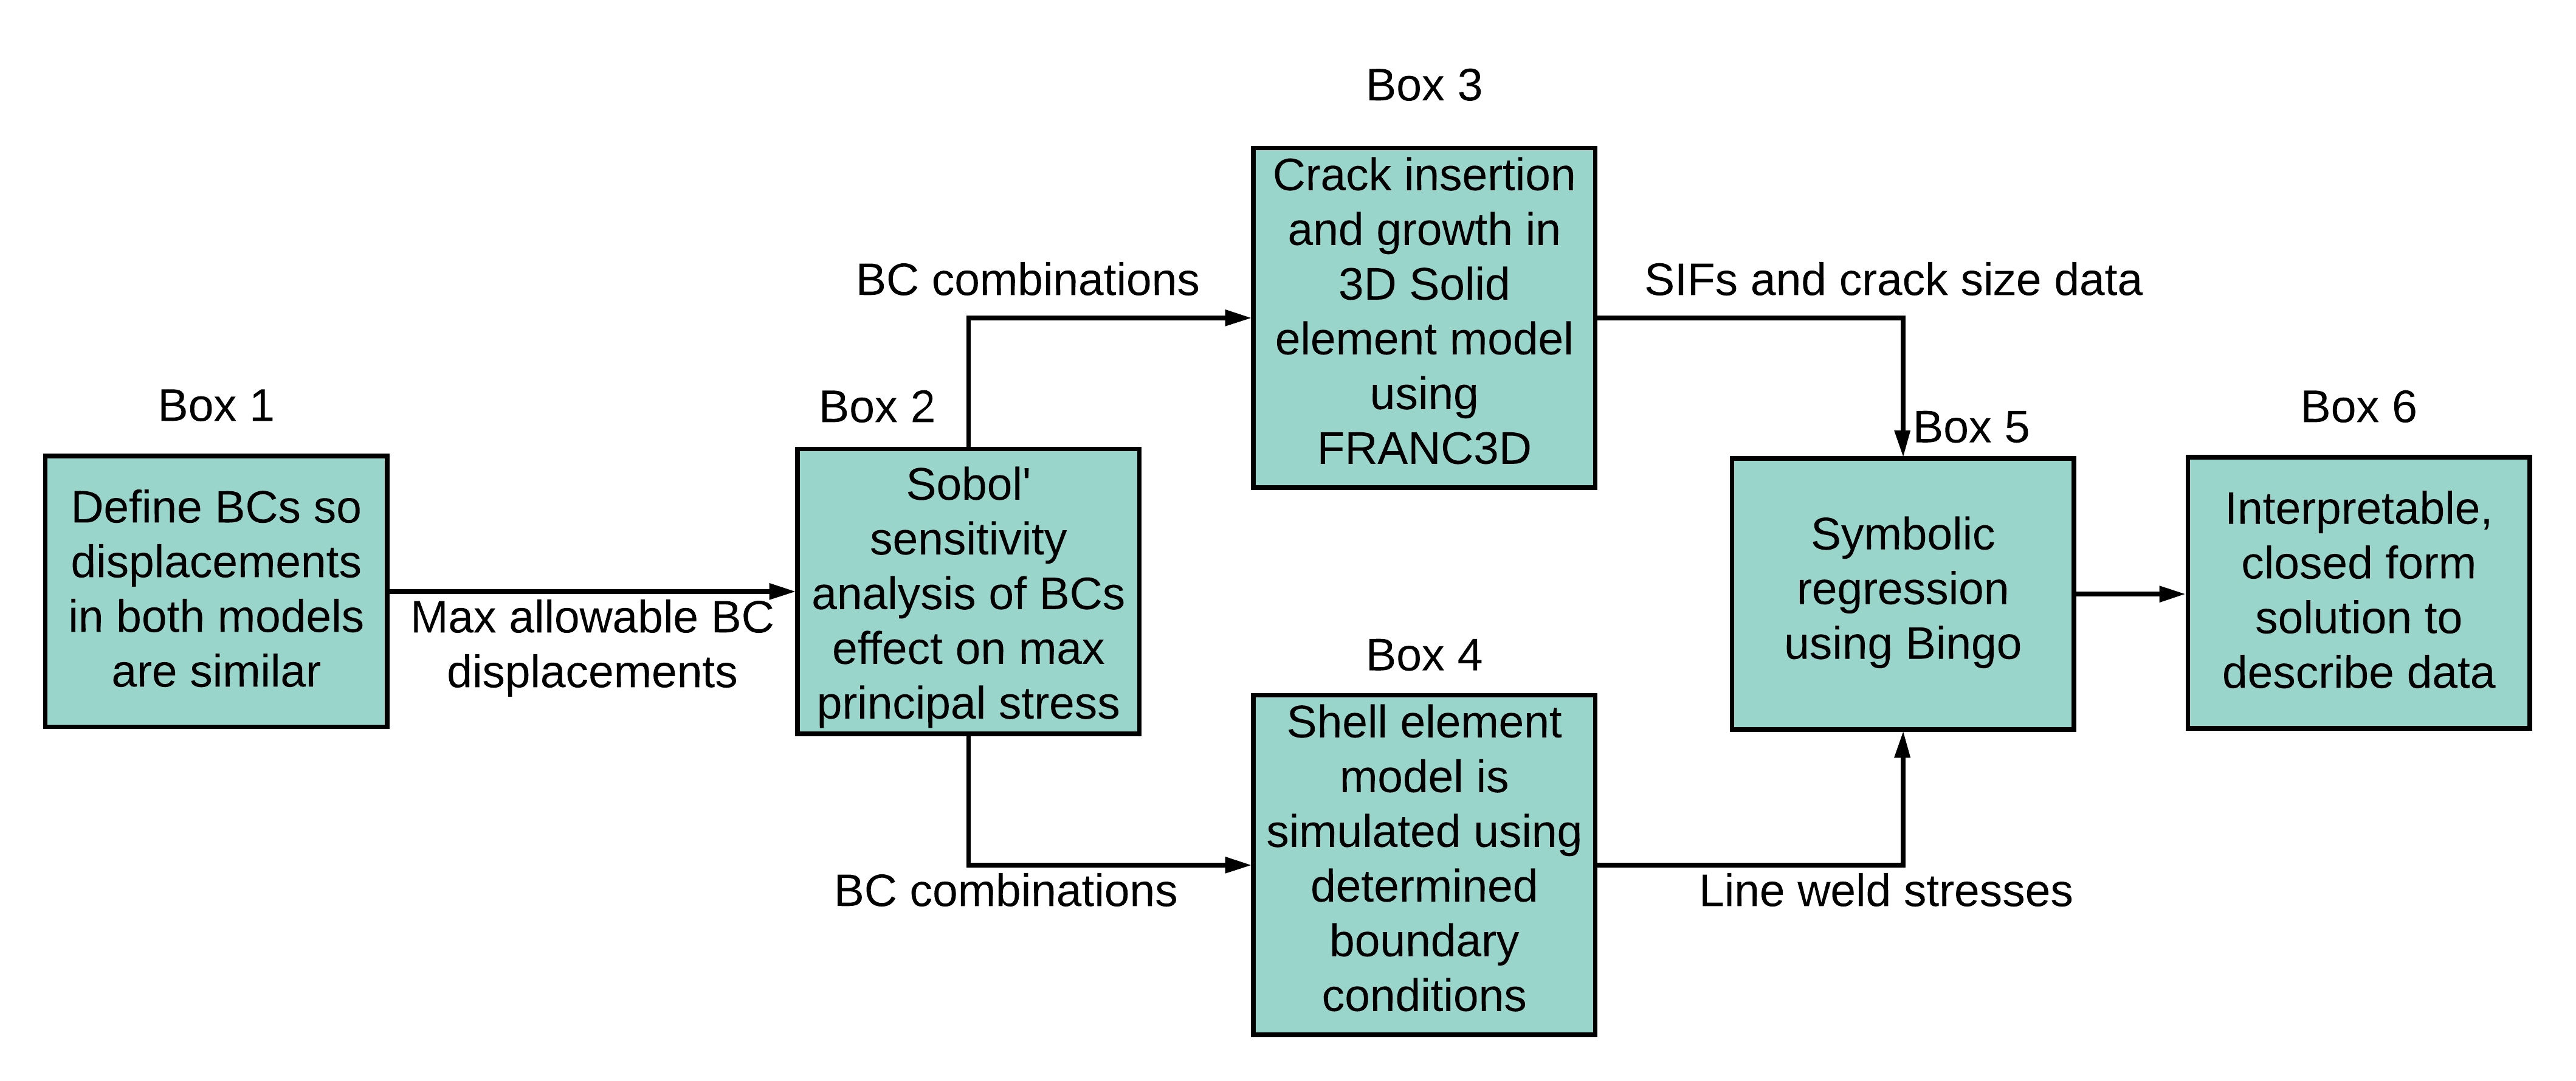
\includegraphics[width=\textwidth,height=\textheight,keepaspectratio]{workflow.png}
\caption{High-level overview of study workflow.}
\label{fig:workflow}
\end{figure}

\begin{figure}[h]
\centering
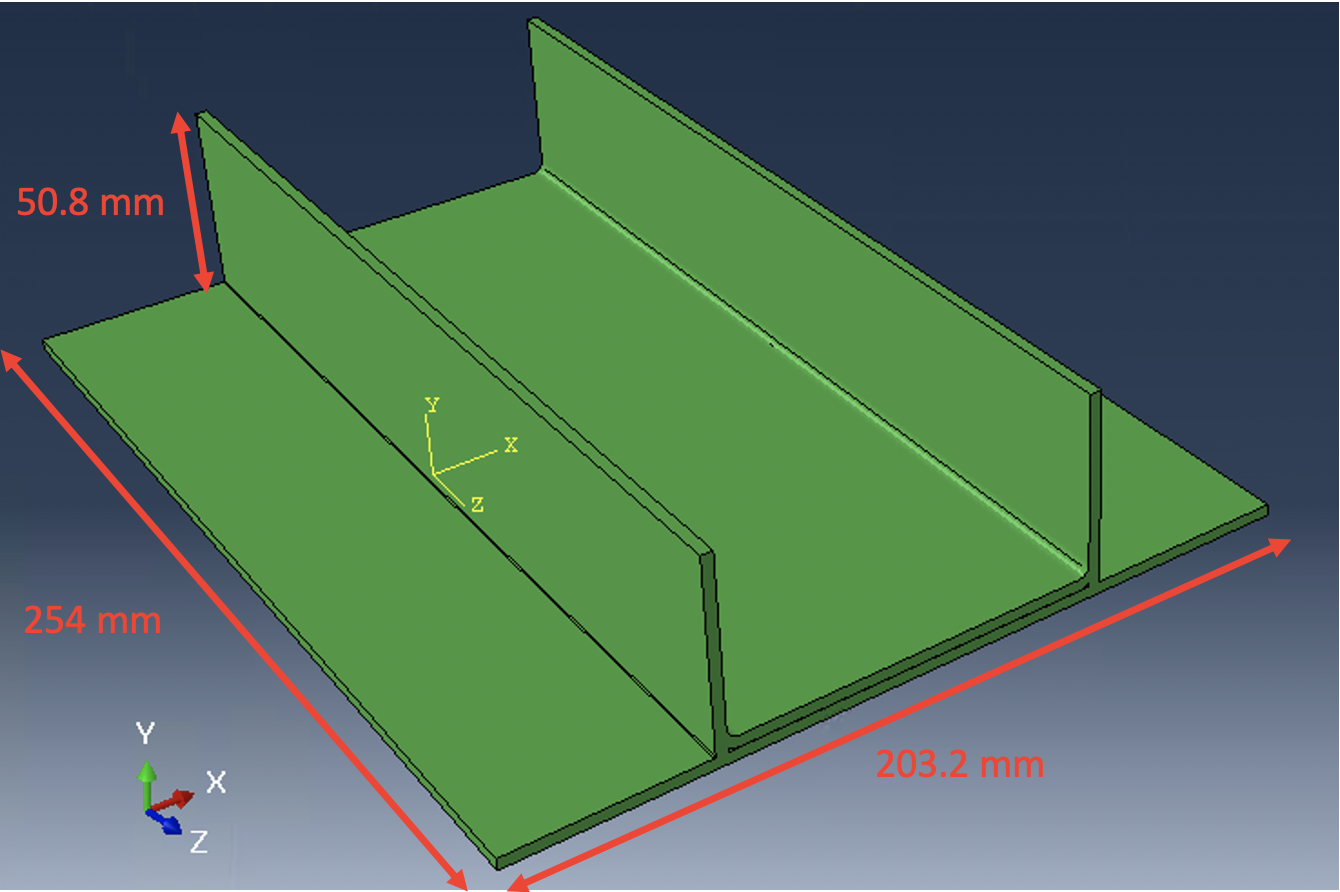
\includegraphics[width=\textwidth,height=\textheight,keepaspectratio]{abaqus_model.png}
\caption{Representation of geometry used to model the C-channel welded to the plate.}
\label{fig:abaqus_model}
\end{figure}

\begin{figure}[h]
\centering
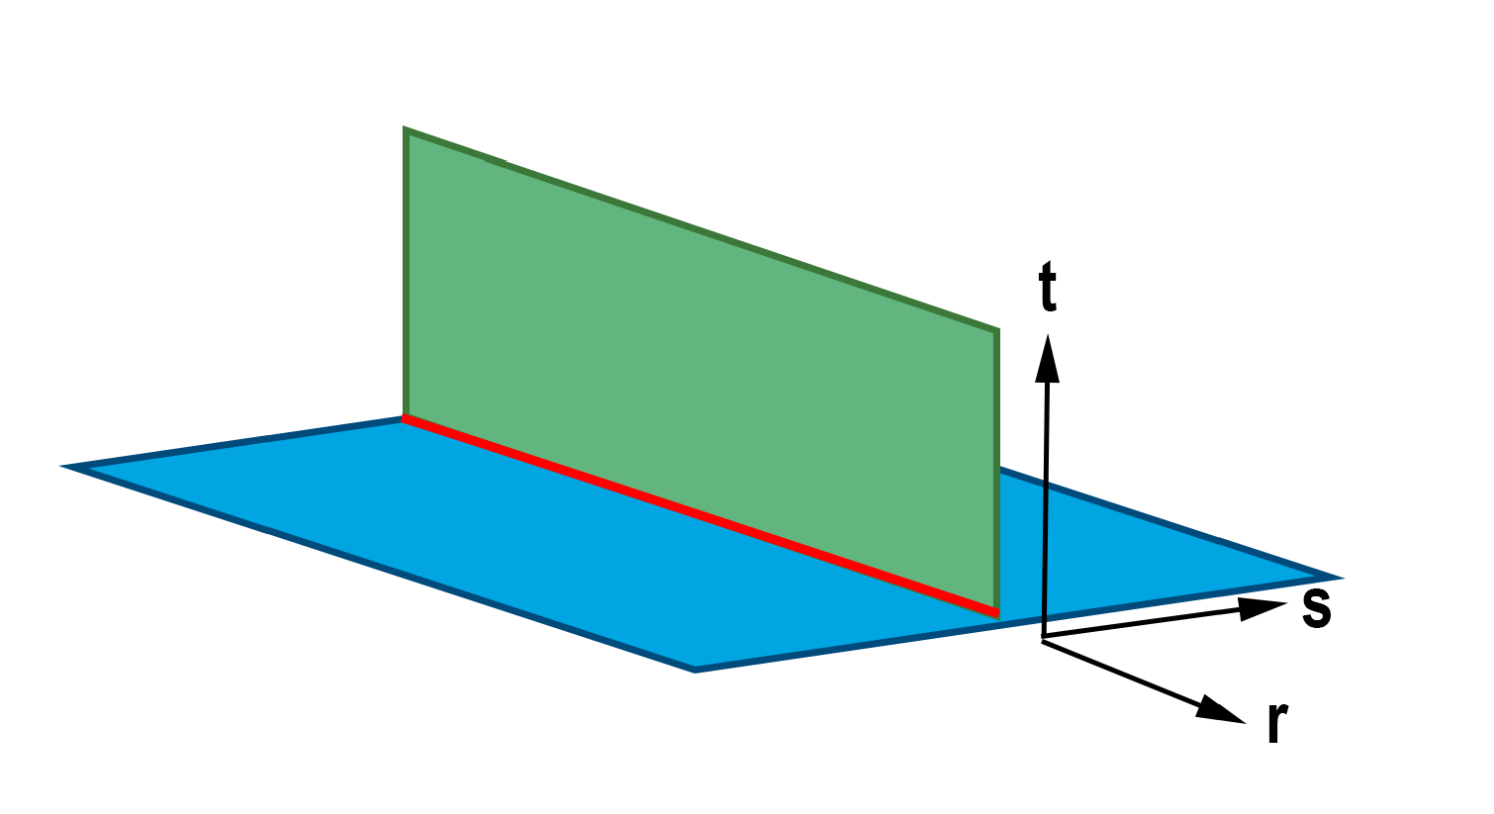
\includegraphics[width=\textwidth,height=\textheight,keepaspectratio]{local_coords.png}
\caption{Illustration of the line-weld local coordinates. The green surface
represents the edge to which the blue surface is welded. The red line represents
the line-weld elements with coordinate axes shown.}
\label{fig:local_coords}
\end{figure}

\begin{figure}[h]
\centering
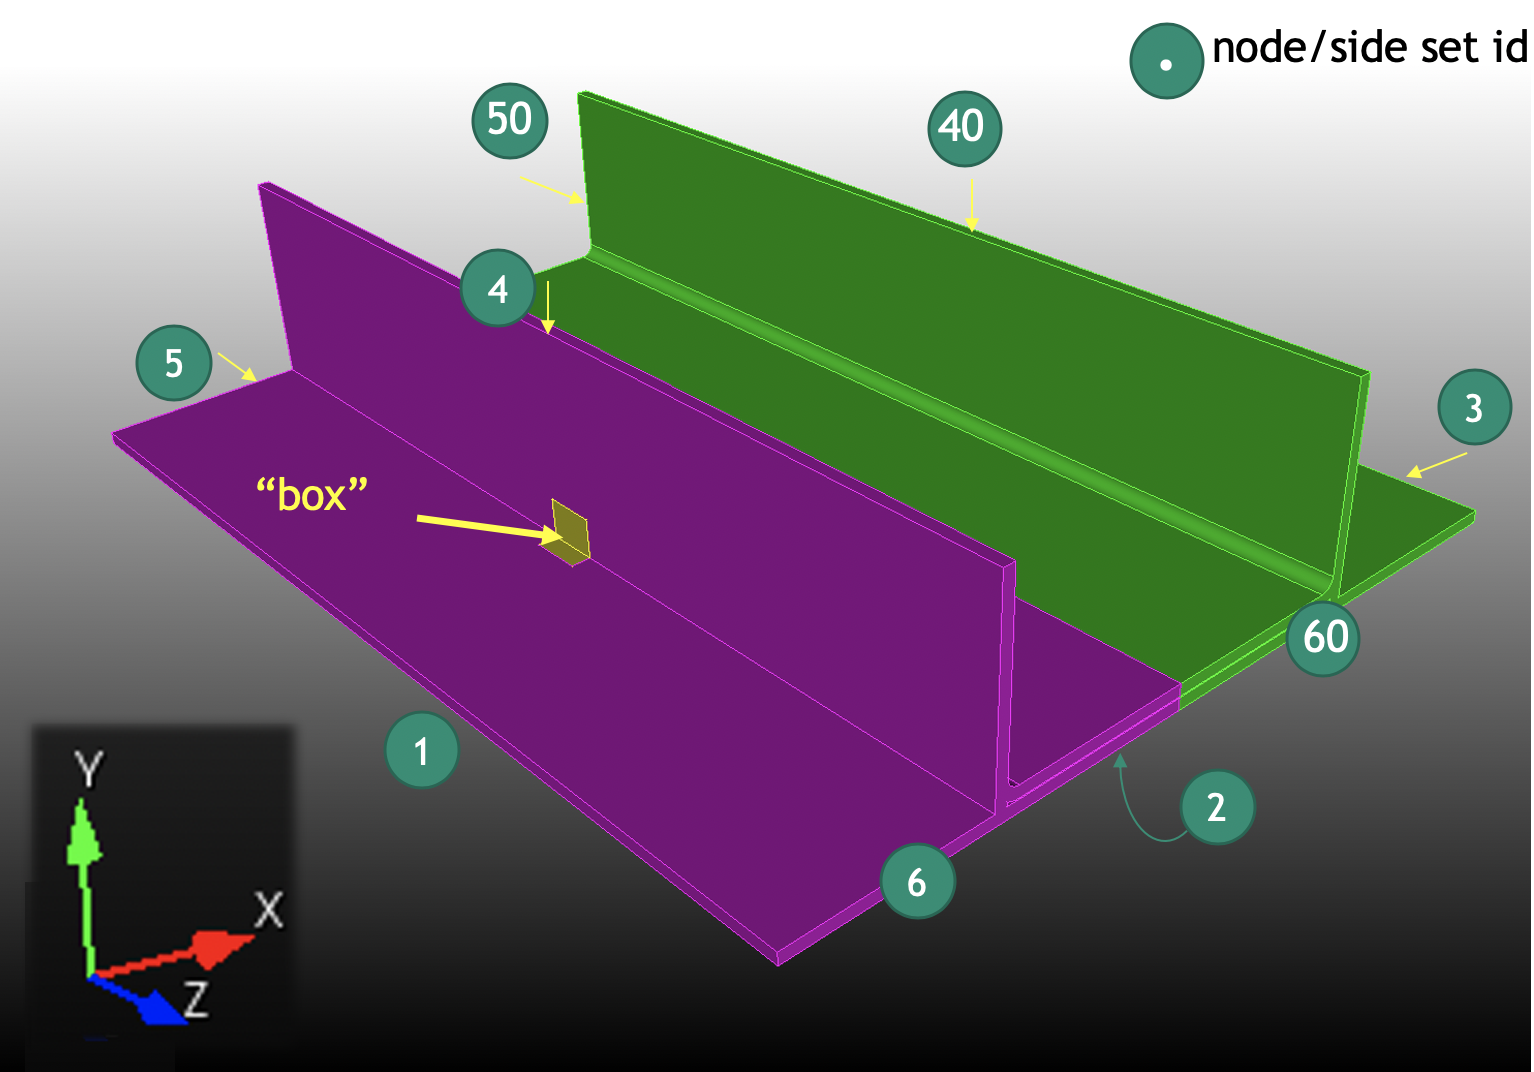
\includegraphics[width=250pt,height=\textheight,keepaspectratio]{surface_numbers.png}
\caption{C-channel welded to a plate with local ``box'' illustrating the local
mesh into which the crack will be inserted. Surface numbers are shown. The
purple and green indicate halves of the model separated by a plane of symmetry.}
\label{fig:surface_nums}
\end{figure}

\begin{figure}[h]
\centering
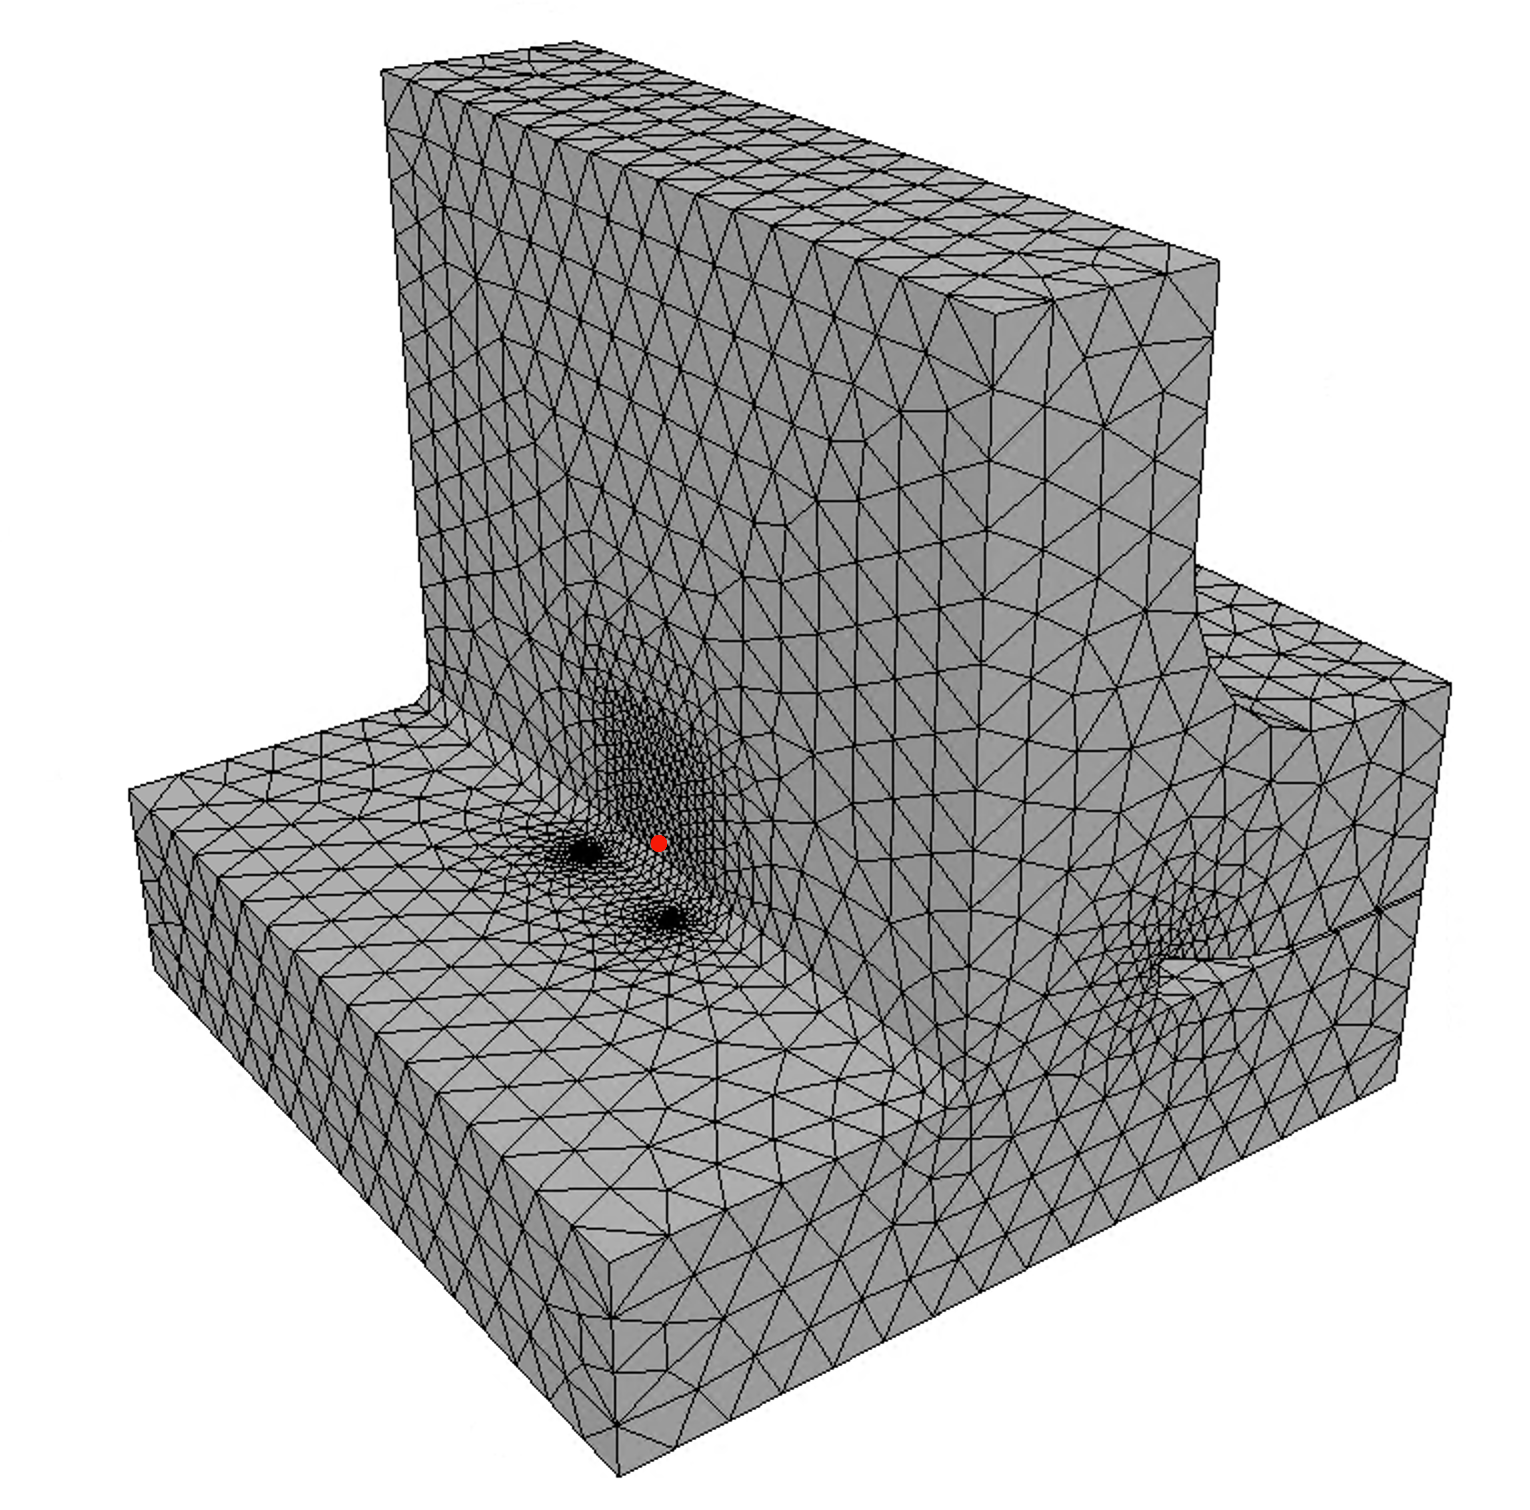
\includegraphics[width=250pt,height=\textheight,keepaspectratio]{local_mps_point.png}
\caption{Local model into which the crack is to be inserted. The maximum principal
stress is calculated at a single point indicated by the red dot. The finer mesh
is shown which facilitates crack insertion.
}
\label{fig:local_mps_point}
\end{figure}

\begin{figure}[h]
\centering
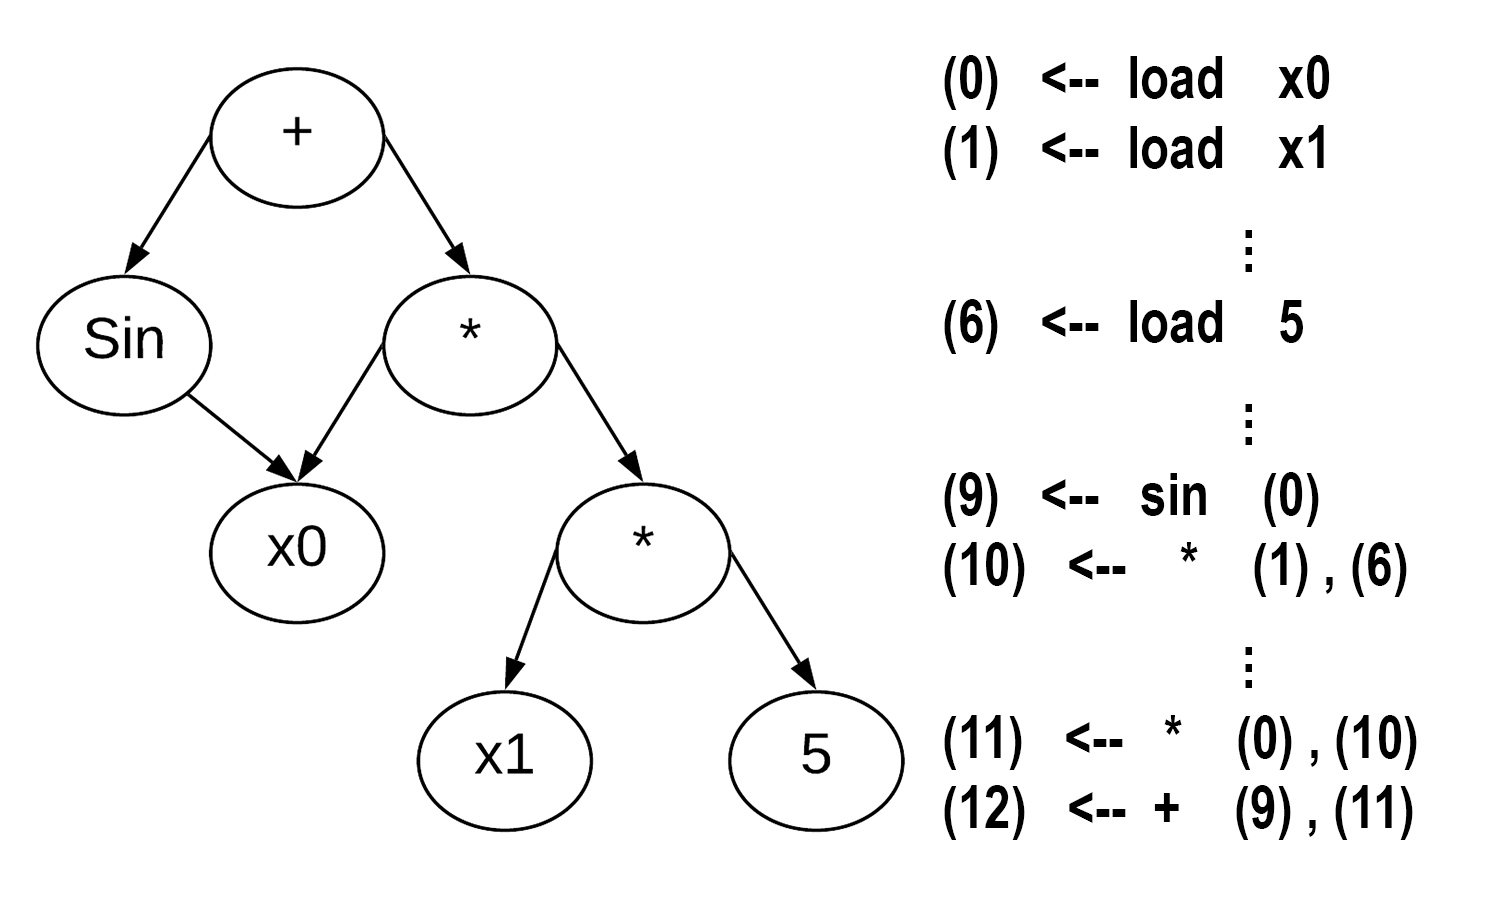
\includegraphics[width=250pt,height=\textheight,keepaspectratio]{agraph.png}
\caption{The equation $f(X) = \sin(x_{0}) + 5*x_{0}*x_{1}$ represented as both a
connected acyclic graph and a list of operations. It's important to note that
the equation is represented without using all nodes in the stack.}
\label{fig:agraph}
\end{figure}

\begin{figure}[h]
\centering
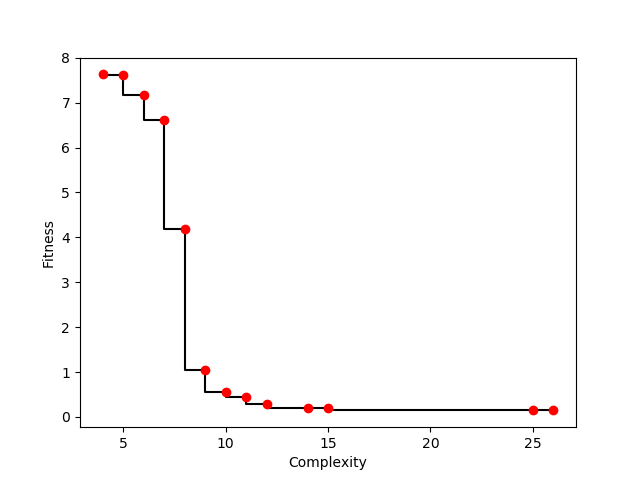
\includegraphics[width=250pt,height=\textheight,keepaspectratio]{pareto_front.png}
\caption{Pareto front of the individuals in a SR population. As complexity
increases, fitness tends to decrease. However, at a certain point, large
increases in complexity do not result in corresponding decreases in error.}
\label{fig:pareto_front}
\end{figure}